\documentclass[11pt]{article}

\usepackage{cite}
\usepackage{graphicx}
\usepackage{amsthm}
\usepackage[english]{babel}
\usepackage{authblk}
\usepackage{array}
\usepackage[T1]{fontenc}
\usepackage[utf8]{inputenc}
\usepackage{parskip}
\usepackage{enumerate}
\usepackage{multirow}
\DeclareGraphicsExtensions{.png}

\title{Survey of the Mobile Application Development}
\author[1]{Andrew Zurn\\Computer Science Department\\Saint John's University\\Collegeville, MN\\awzurn@csbsju.edu}

\begin{document}
\maketitle
\begin{abstract}
\noindent The mobile application development environment has seen many large shifts in the way developers have gone about creating applications, originating from mobile web applications, to native development, and now into a new field of hybrid development.  This hybrid approach to building cross-platform applications, which mainly leverages the web technology stack (HTML5/CSS/JavaScript) and also platform-specific software development kits (SDK), is becoming a viable solution for developers that are looking to maintain a single code base that ports to many target environments.  Research has been done in this field, some of which shows promising results in the eventual adoption of they hybrid solutions for developing mobile applications that will achieve the look and feel of their native predecessors.
\end{abstract}

\section{Introduction}
\setlength{\parindent}{.75cm}
Mobile application development has been a large issue across the industry, and comes in many forms and facets.  This area has seen various approaches since it's forthcomings, which date back all the way to the late 1990s.  Many early entities in the mobile app environment built closed systems like PalmOS and Windows Mobile~\cite{Dediu2011}, but it was in 1998 that Java Micro Edition (J2ME) was introduced.  Although J2ME was originally meant to bring new options for developers wanting to target multiple devices, it wasn't long before the major entities in the mobile arena, like Google, Apple, BlackBerry, and Microsoft, introduced their own software development kits (SDKs), all greatly varying in platform development tools, languages, frameworks and methodologies, in addition to only targeting their own particular devices.~\cite{Corral2011}\\

\indent However, there is a new trend in the mobile development spectrum, where developers are beginning to build their applications with the goal of cross-compatibility in mind.  Initially, effort was done in developing what many call mobile web applications, which leveraged web technologies like HTML5 and CSS that would be run inside a mobile device’s web browser.~\cite{Leroux2011}  However, an even newer adaptation for mobile development has emerged in the last few years, that is the “hybrid” approach, which connects the best aspects of native and web-based software development, where developers can build applications that mainly use HTML5, CSS, and JavaScript, but are wrapped into a native-like application.~\cite{Xanthopoulos2013}  In this paper, a glance of the history of mobile application development, and also an analysis of the research being done in this area known as 'hybrid' development will be presented.\\

\section{Survey}
\subsection{History of Mobile Web Development}
\indent This mainly web-based hybrid development solution, although gaining popularity in the last year or two, actually isn't an entirely new concept.  Steve Jobs, in his original announcement of the iPhone in 2007, was only going to let developers create third-party application for the phone's web browser (although shortly after that they joined the rest of leaders in mobile development by releasing their SDK for iPhone development.) ~\cite{Mims2013}  Although developing mobile web applications has long since been an option for developing application targeted towards web applications, it does have its limits in providing a viable alternative to native applications.  In their article, Viktor Kolokolov and Paul Baumann, researchers at the Wireless Sensor Network(WSN) Lab at the Technische Universität Darmstadt, provides critical insight into the advantages and also the limits of this technology. They state that "the key advantage of web applications over natively build mobile applications is their cross-platform compatibility. Yet, web application are often hampered by the limited capabilities of mobile browsers and cannot access low-level hardware and software resource of the hosting devices." ~\cite{Kolokolov2013}  It is this reason that mobile web applications, at the time of the introduction of the first generation of smart phones around 2007, drove many mobile leaders towards introducing their development platforms to specifically target their own devices.

\subsection{A New Shift from Native Development}
The main motivator in proliferation away from native SDKs, is in main part, driven by the cost, time, and the immense code base associated with building each application for their respective platforms. Luis Corral, a researcher at Free University of Bonzen/Bolzano, points out the major fallacy in native development, stating that 

\begin{quote}
If a developer wants to deploy his application in more than one platform, it is necessary to translate the original source code to the adequate one, as well adapting APIs and low-level implementations so that the new target could support the application in the way it was conceived in the original platform.  After that, it is compulsory to rebuild the application to obtain the proper executable code. ~\cite{Corral2011}
\end{quote}

Essentially, if a develop wants to port their application, they in large part have to reproduce a great amount of their code, test and insure the user experience of the new application is comparative to the original application, and also have to maintain the two distinct code bases beyond that.\\

Although the status quo of developing mobile applications mainly with a platform-specific SDKs has grown quite popular and is always seeing new developments, a few, such as Corral and Kolokolov, believe we will see a massive shift from native development, to more web-based and 'hybrid' approaches.  Spyros Xanthopoulos and Stelios Xinogalos of the Aristotle University of Thessaloniki and the University of Macedonia exclaim that the ultimate goal of this shift towards cross-platform  mobile app development is to achieve native app performance and run on as many platforms as possible. They go onto state that "the concept of {\it write once, run anywhere} can't be applied when building native applications, the best alternative option for companies is the {\it cross-platform mobile development}, Cross-platform development simplifies the maintenance and deployment processes, and saves development time and effort."  ~\cite{Xanthopoulos2013}\\

\subsection{The 'Hybrid' Solution}
The solution that many seem to see the industry moving towards is the aforementioned hybrid solution.  Although these applications are not yet a total replacement for native applications yet in terms of performance and user experience, they are a more viable option than building multiple native applications, and allow for more access to device's powerful hardware and various features.  As can be seen in Figure 1, hybrid applications rate just as well as native applications in mostly all of the important aspects to consider when building a mobile application, and only really lacks in the performance area.\\


\begin{figure}[h]
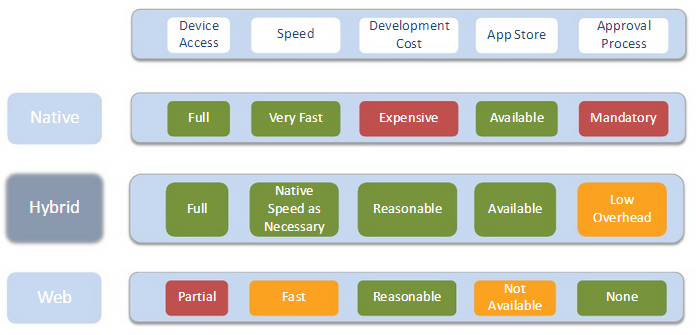
\includegraphics[scale=0.7]{ComparativeTable}
\caption{Comparative analysis of cross-platform and native development approaches ~\cite{Kaminitz2011}}
\end{figure}

Brian Leroux and Andrew Charland, writers for {\it Communications of the ACM} provide a brief explanation in their article, "Web Application Development: Web vs. Native," where they critic a development platform called {\it PhoneGap}.  They state

\begin{quote}
PhoneGap is an open source framework that provides developers with an environment where they can create apps in HTML, CSS and JavaScript and still call native device features and sensors via a common JS API.  The PhoneGap framework contains the native-code pieces to interact with the underlying operating system and pass information back to the JavaScript app running in the Webview container. ~\cite{Leroux2011}  
\end{quote}




{\it PhoneGap} is only one of many platforms that allows for this development of mobile web applications that can access the lower-levels of a phone's rich features.  Among some other notable platforms, of which have also had research done on and published on them are {\it Accelerator Titanium} ~\cite{Xanthopoulos2013}, {\it Cabana} ~\cite{Dickson2012}, {\it Lively for Qt} ~\cite{Mikkonen2009}, and {\it MD2} ~\cite{Heitkoetter2013}.  Xanthopoulos and Xinogalos offer valuable insight into some of these development platforms, allowing for us to see exactly how powerful these hybrid applications can look and feel, and how they are quite possibly the solution for the problem of developing multiple native applications. They state,

\begin{quote}
If default native look and feels is necessary then the implementation of interpreted(hybrid) apps is the best option.  A popular development environment for building interpreted(hybrid) apps is Titanium... PhoneGap is one of the dominant development environments for building hybrid apps.  Frameworks like Titanium and PhoneGap are using widely used web development technologies (especially JavaScript), do not require a detailed knowledge of the target platform and are certainly worth considering for building cross-platform applications.  Titanium supports the operating systems iOS, Android and BlackBerry, while supported operating systems by PhoneGap include iOS, Android, Blackberry, Windows Mobile and more.
\end{quote}

As they go onto state, these two areas are both highly "promising", and as many seem to think, are highly viable solutions for developers looking to code once and deploy across a variety of platforms.~\cite{Xanthopoulos2013}

\section{Conclusion}
The field of mobile development, if taken from it's more recent beginnings in 2007, has been an area that has seen massive shifts in its development paradigms and approaches.  Building mobile applications has in large part become a problem for companies needing to create their applications for various platforms, and although building apps completely out of HTML5 and CSS poses a solution for the problem of cross-compatibility, it lacks the feel and performance of native applications.  This is where the recent shift towards applications developed using frameworks like {\it Appcelerator}, {\it PhoneGap}, and others, has given programmers the ability to create a single code base that build native applications for a majority of platforms, such as iPhone, Android, and BlackBerry.  These hybrid applications have the potential to be a great alternative for native applications, and will more than likely, as many researchers believe, continue to grow in popularity for years to come. Ultimately, as Leroux and Charland exclaim 

\begin{quote}
The web technology stack has not achieved the level of performance we can attain with native code, but it's getting close.  We're confident that Web technologies will become indistinguishable from native experiences.  In the meantime, Web developers must focus on delivering data while working diligently on improving the decor.  As much as native and Web are pitted against one another in this debate, the likely outcome is a hybrid solution. ~\cite{Leroux2011}
\end{quote} 

\bibliographystyle{plain}
\bibliography{SurveyPaperBibliography}
\end{document}